\documentclass[tikz]{standalone}

\begin{document}
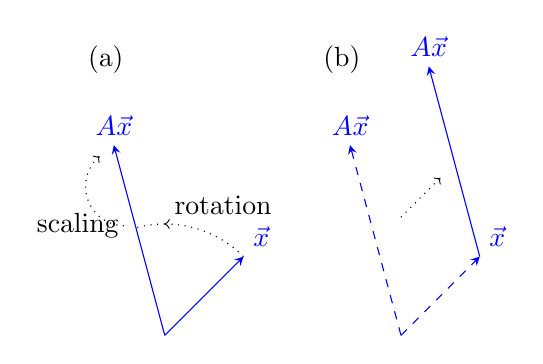
\begin{tikzpicture}
  \begin{scope}[xshift=0]
    \node at (-0.75,3.5) {(a)};
    \draw[->,>=stealth,blue]
      (0,0)--(1,1) node[above right] {\(\vec{x}\)};
    \draw[variable=\t, samples=50, domain=45:90,dotted,->]
      plot( {1.4142*cos(\t)},{1.4142*sin(\t)} ) node[above right] {rotation};
    \draw[variable=\t, samples=50, domain=90:105,dotted]
      plot( {1.4142*cos(\t)},{1.4142*sin(\t)} );
    \draw[variable=\r, samples=20, domain=0:2.5,->,>=stealth,blue]
      plot( {\r*cos(105)}, {\r*sin(105)} ) node[above] {\(A \vec{x}\)};
    \draw[variable=\t, samples=50, domain=-230:-85,<-,dotted]
      plot( {1.957*cos(105) + 0.5*cos(\t)}, {1.957*sin(105) +0.5*sin(\t)} ) node[left] {scaling};
  \end{scope}
  \begin{scope}[xshift=3cm]
    \node at (-0.75,3.5) {(b)};
    \draw[->,>=stealth,blue,dashed]
      (0,0)--(1,1) node[above right] {\(\vec{x}\)};
    \draw[variable=\r, samples=20, domain=0:2.5,->,>=stealth,blue,dashed]
      plot( {\r*cos(105)}, {\r*sin(105)} ) node[above] {\(A \vec{x}\)};
    \draw[variable=\r, samples=20, domain=0:2.5,->,>=stealth,blue]
      plot( {1 + \r*cos(105)}, {1+\r*sin(105)} ) node[above] {\(A \vec{x}\)};
    \draw[dotted,->] (0,1.5)--(0.5,2);
  \end{scope}
\end{tikzpicture}
\end{document}
